\documentclass{beamer}

\usepackage{listings}  % Package to include python syntax code
\usepackage{color} % Package to include colors for syntax highlighting
\usepackage{graphicx}  % Package to include images
\usepackage{hyperref}  % Hyperlinks
\usepackage{tikz}
\usepackage{graphics}

\lstset{  % Settings for listings package
    backgroundcolor=\color{cyan!10},  % Includes a light blue background color
    numbers=left,  % Includes line numbers
    keywordstyle=\bfseries\color{green!40!black},  % Bold and color green for keywords
    identifierstyle=\color{blue},  % Other words are colored blue
    stringstyle=\color{orange},  % Strings are orange
    showstringspaces=false  % Don't show spaces in strings
}

\setbeamertemplate{navigation symbols}{}  % Remove navigation symbols

\title{Computing for Mathematics: Week 1}
\date{}


\begin{document}

\frame{
    \begin{center}
        \Huge Mid module Feedback 2014-2015
    \end{center}
}

\frame{
    \begin{center}
        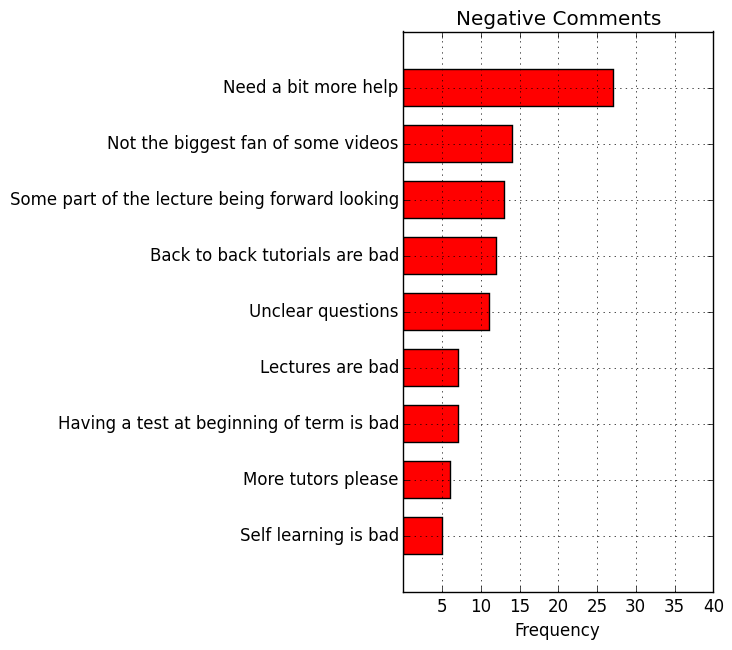
\includegraphics[width=\textwidth]{negative-2014-2015.png}
    \end{center}
}

\frame{
    \begin{center}
        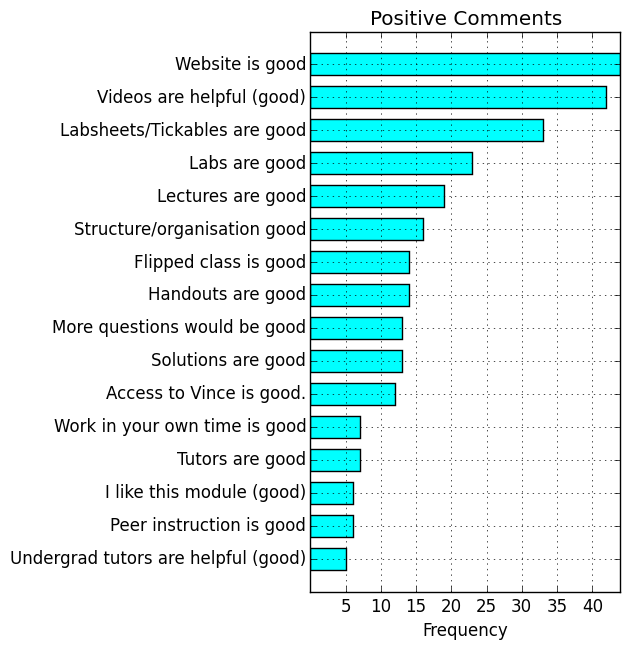
\includegraphics[width=\textwidth]{positive_2014-2015.png}
    \end{center}
}

\frame{
    \frametitle{Interesting}
    \begin{quote}
        ``More emphasis on teaching rather than assessing.''
    \end{quote}
}

\frame{
    \frametitle{Helpful}
    \begin{quote}
        ``No matter how difficult the lab sheets are, it always feels like there is sufficient support, either from Vince or from various online resources.''
    \end{quote}
}

\frame{
    \frametitle{Helpful}
    \begin{quote}
        ``Hours where the lecturer is available to help students are immediately after the deadline and probably before a student has started the next week's work.''
    \end{quote}
}

\frame{
    \frametitle{Helpful}
    \begin{quote}
            ``Would like to know about all assessment from the start, class test was only recently revealed and don't know much about the remaining 45\%''
    \end{quote}
}

\frame{
    \frametitle{Helpful}
    \begin{quote}
        ``Having a better idea of which parts of alternative resources relate to each week could make them more helpful (save time searching through what is often a very large and confusing source of information.''
    \end{quote}
}

\frame{
    \frametitle{Helpful}
    \begin{quote}
        ``Introductory handout for software''
    \end{quote}
}

\frame{
    \frametitle{Helpful}
    \begin{quote}
        ``Have the lecture run till the end for those who need help.''
    \end{quote}
}

\frame{
    \frametitle{Helpful}
    \begin{quote}
        ``Lecturer is quite intimidating although helpful when questions are asked. Puts me off asking questions, pushes me towards just copying other students code.''
    \end{quote}
}

\frame{
    \frametitle{Helpful}
    \begin{quote}
        ``Only one video tutorial is given providing only one angle''
    \end{quote}
}

\frame{
    \frametitle{Helpful}
    \begin{quote}
        ``More Mathematics related (more sage less python)''
    \end{quote}
}


\frame{
    \frametitle{About the methodology}
    \begin{quote}
        ``Office hours are the same time as lectures/tutorials.''
    \end{quote}
}

\frame{
    \frametitle{About the methodology}
    \begin{quote}
        ``Classroom atmosphere in labs, please.''
    \end{quote}
}

\frame{
    \frametitle{About the methodology}
    \begin{quote}
        ``I think it would be effective if maybe the first tutorial of the 2 could be a 'teaching' tutorial as I find learning some concepts hard.''
    \end{quote}
}

\frame{
    \frametitle{About the methodology}
    \begin{quote}
        ``People able to complete tickables without understanding what they have done - just using code from video or copy and paste''
    \end{quote}
}

\frame{
    \frametitle{Quirky}
    \begin{quote}
        ``More compulsory tickables as its easy to just not do them.''
    \end{quote}
}

\frame{
    \frametitle{Quirky}
    \begin{quote}
        ``Stop waiting for people not to talk: wasting my time!''
    \end{quote}
}

\frame{
    \frametitle{Quirky}
    \begin{quote}
        ``Jason. \#awesome''
    \end{quote}
}

\frame{
    \frametitle{Quirky}
    \begin{quote}
        ``Vince, Smile! :)''
    \end{quote}
}

\frame{
    \frametitle{Quirky}
    \begin{quote}
        ``I'm not a cat person.''
    \end{quote}
}

\frame{
    \frametitle{Quirky}
    \begin{quote}
        ``Free Pen-Drives would be nice\ldots''
    \end{quote}
}

\end{document}
